
% ############### PRODUCT PERSPECTIVE ####################à
\subsection{Product perspective}
\hyperref[tab:acronymsTable]{DREAM} is a functional multi-user software platform whose purpose is to provide functionalities described in section \ref{sect:product_functions}. The system will be composed by a series of software and hardware interfaces that interact in such a way to let users manipulate shared data. It also will exploit some graphical interface packages in order to be user friendly and easy to use.
This product is designed to run on a wide variety of machines, including operating systems Mac OS, Windows, Linux, Android and iOS. 

\begin{figure}[H]
	\centering
    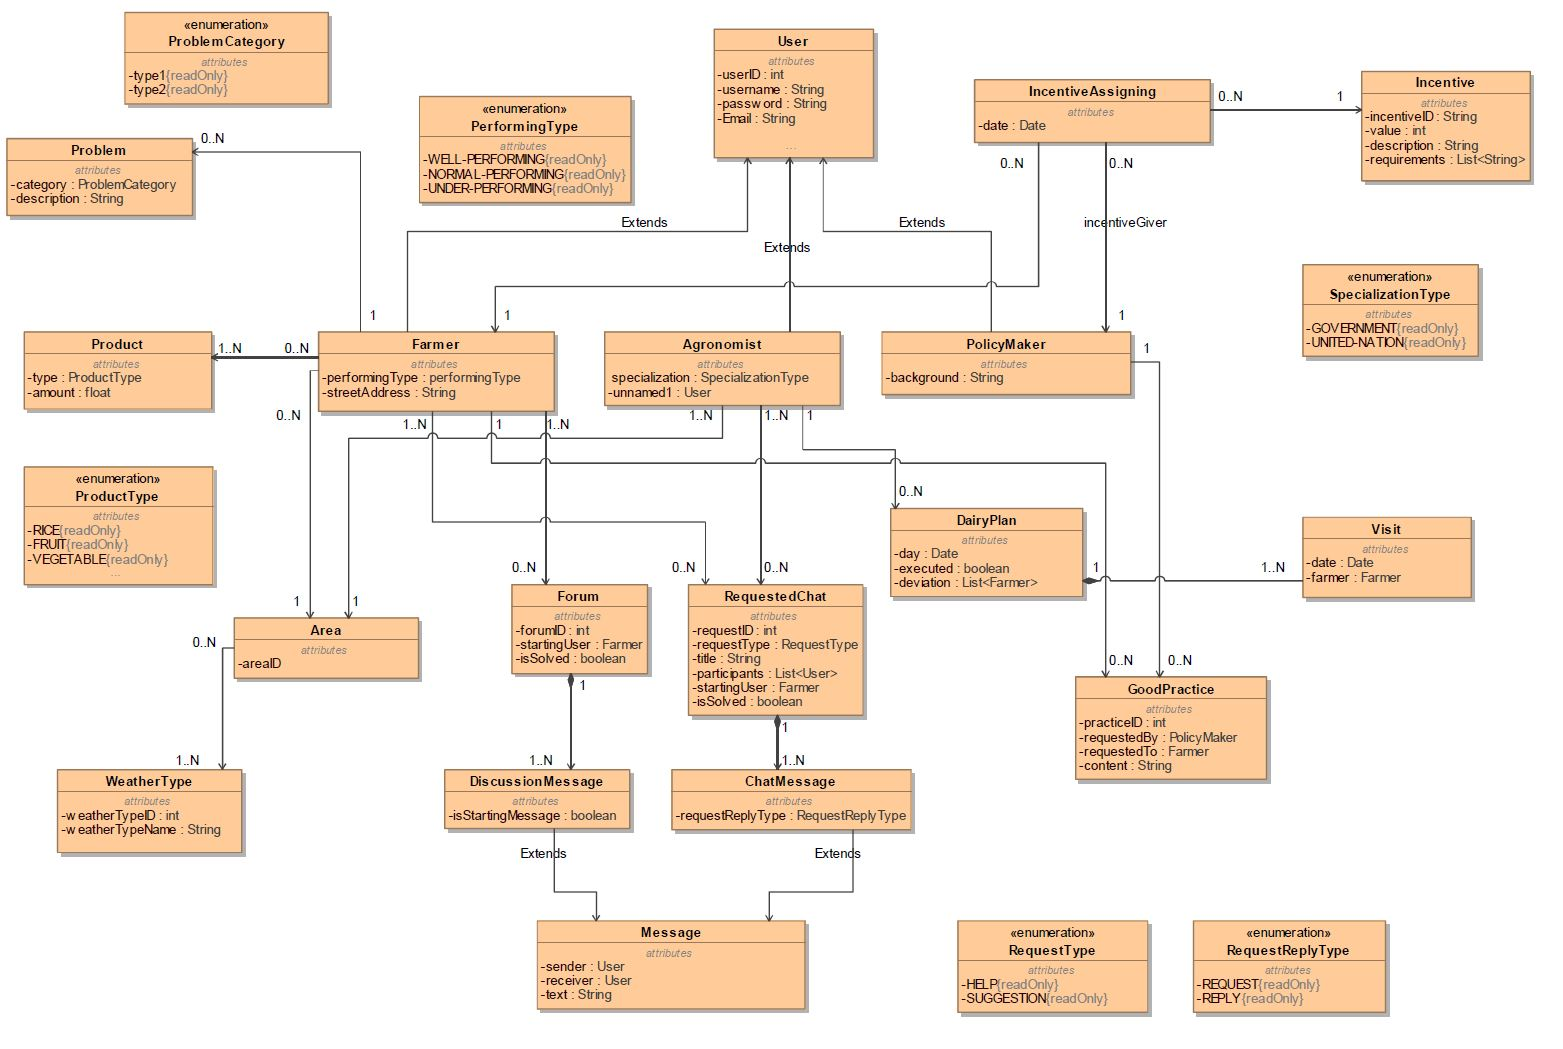
\includegraphics[page=1, width=\textwidth]{Images/uml_draft.JPG}
	\caption{\label{fig:uml_class_diagram}High level UML diagram}
\end{figure}

\subsubsection{User interfaces} % TODO revise the verbs
\label{sect:user_interfaces}
According to the assignment document, the system will interact with 3 different user classes: policy makers, farmers and agronomists. In order to be more accessible and to fulfill the user needs, the application will be supported by different devices. These users should interface to the service through electronic devices with an internet connection. Users that need to access the service will have the possibility to connect through:
\begin{itemize}
    \item an internet browser, addressing a specific web domain (such as \textit{www.dream.com}) that permits users to sign up/in a dedicated web application;
    \item a mobile application that can be installed on smartphones or tablets (both iOS and Android).
\end{itemize}


\subsubsection{Software interfaces}
In order to improve software flexibility and quality, \hyperref[tab:acronymsTable]{DREAM} will use a set of external software interfaces. Rather than providing names of real specific services, we consider reasonable referring to them as functionalities to be later defined in the design phase:
\begin{description}[font=~\normalfont\scshape]
    \item[\textbf{\textcolor{myblue}{universal logins}}] \hfill \\login \hyperref[tab:acronymsTable]{APIs} that also provide access by using their Facebook, Twitter, or Google profile login details are good candidates in order to quickly autenthicate the user while guaranteeing security;
    \item[\textbf{\textcolor{myblue}{big data manipulation}}] \hfill \\since a wide quantity of information needs to be recorded and accessed in a distributed system fashion, \hyperref[tab:acronymsTable]{DBMS} \hyperref[tab:acronymsTable]{APIs} are necessary for data extraction performances optimization;
    \item[\textbf{\textcolor{myblue}{third party payment processing}}] \hfill \\for guaranteeing secure payment transactions online payment \hyperref[tab:acronymsTable]{APIs} such as PayPal should be used;
    \item[\textbf{\textcolor{myblue}{third party data science research}}] \hfill \\% TODO
\end{description}

\subsubsection{Hardware interfaces \& constraints}
DREAM system will be composed by multiple different hardware components which can be described from two points of view:
\begin{description}[font=~\normalfont\scshape]
    \item[\textbf{\textcolor{myblue}{user perspective}}] \hfill \\Since \hyperref[tab:acronymsTable]{DREAM} platform is accessed by users in a fully virtual fashion, the minimum required hardware interfaces are the ones that provides internet connection, input components, a screen to visualize \hyperref[tab:acronymsTable]{GUI} and a web browser or an application store (like smartphones, personal computers, tablets and smart TVs).
    \item[\textbf{\textcolor{myblue}{system perspective}}] \hfill \\According to the assignment, the system should be composed by hardware devices designed to gather Telangana's environment information such as soil humidity sensor and the ones responsible for the predefined water irrigation system.
\end{description}
The user hardware interfaces also represent constrains that are required in order to permit the users to interact with the systems and manipulate shared data.

\subsection{Product functions}
\label{sect:product_functions}
In this section the main functionalities of the \hyperref[tab:acronymsTable]{S2B} are presented, described and enriched with \hyperref[tab:acronymsTable]{BPMN} diagrams in order to guarantee an higher level of understanding.
\subsubsection{Sign up}
This functionality allows the user to create an account to access the platform.
Firstly he opens the sign up page and fills the information required such as email, address etc.
Then, if the inserted data is accepted, an e-mail is sent to the User asking for their verification.
Lastly, if all the steps above are done, the user is redirected to the login page.

\begin{figure}[H]
	\centering
    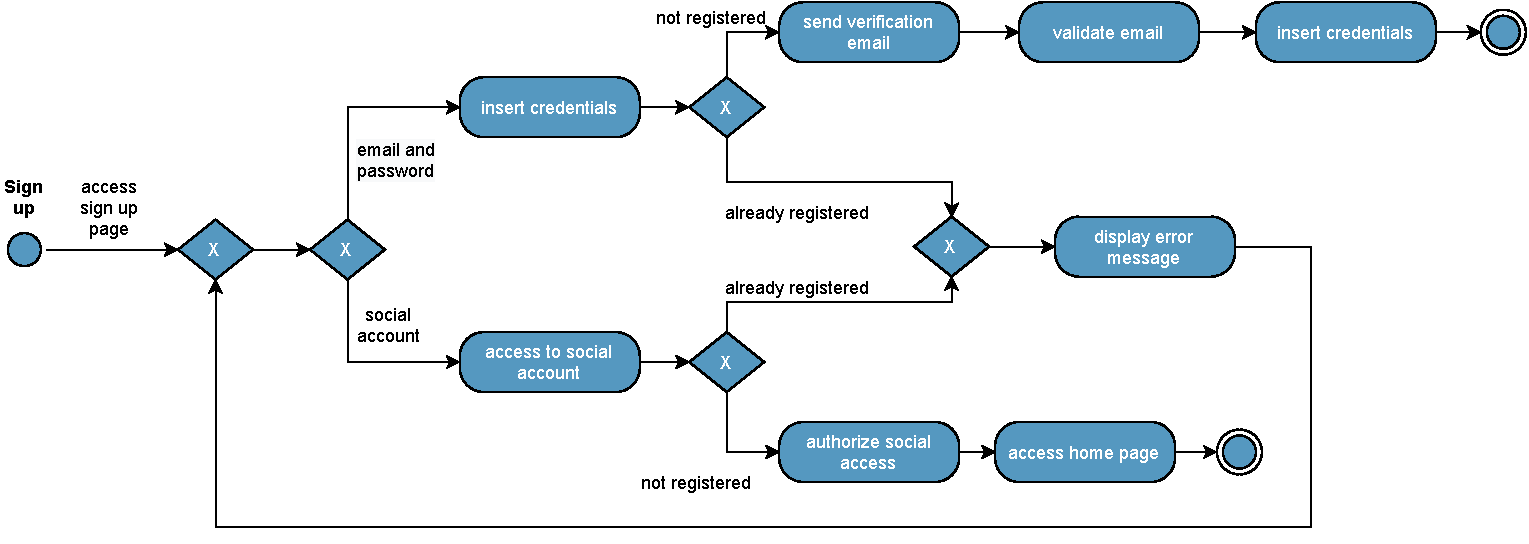
\includegraphics[width=\textwidth]{Images/BPMN/signup.pdf}
	\caption{\label{fig:bpmn_sign_up}BPMN diagram of sign Up}
\end{figure}

\subsubsection{Sharing issues to get help and suggestions}
This functionality is available for farmers and agronomists. The farmer selects the request section and the system displays the send request button; if it is clicked, all the saved contacts are shown. After selecting to whom to ask, insert the question in the text form, presses send button, then the request is sent successfully.


\begin{figure}[H]
	\centering
    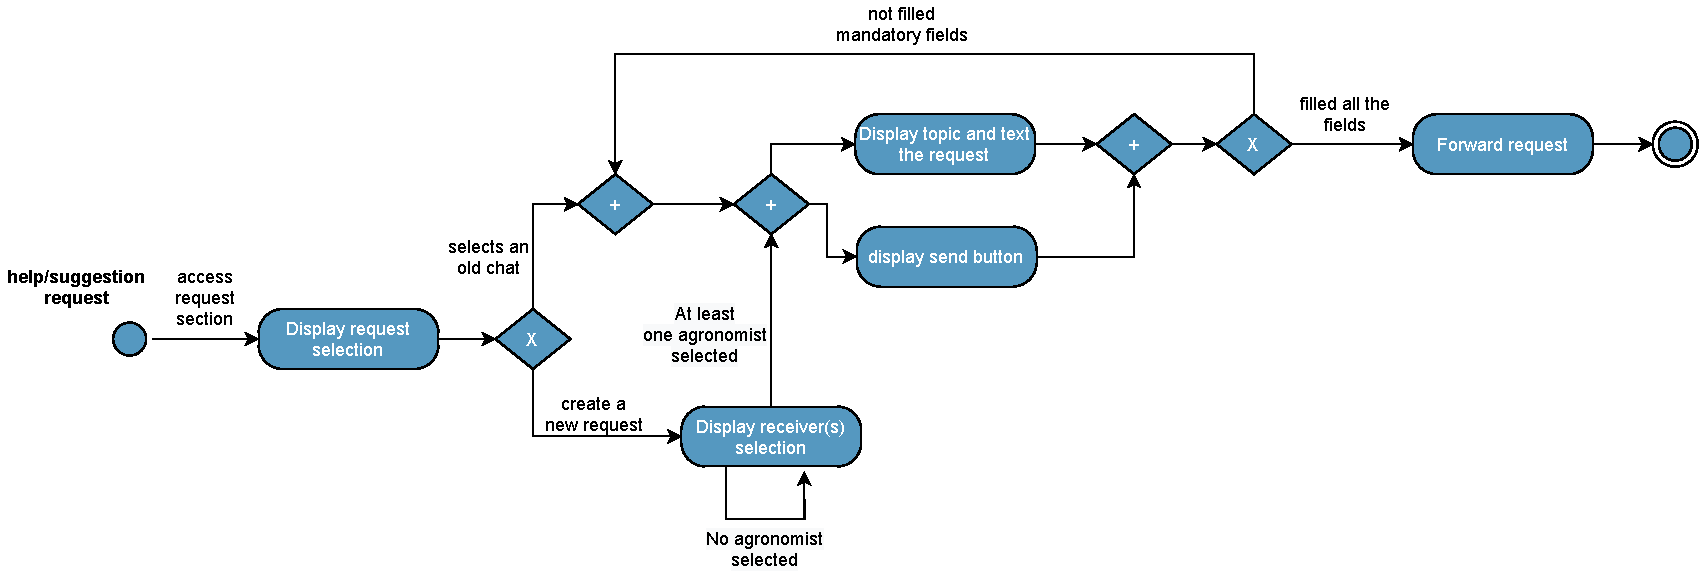
\includegraphics[width=\textwidth]{Images/BPMN/help-suggestion-request.pdf}
	\caption{\label{fig:bpmn_request}BPMN diagram of help/suggestion request}
\end{figure}


\subsubsection{Communication (among farmers) on forums}
This functionality is required for allowing farmers to exchange their opinions. The farmer accesses the forum section which presents an eventual list that contains both previous submitted forums and farmer’s forum replies. By selecting forum upload button, the system displays 
insertion form containing topic/context of the thread, title and question content. If the farmer 
inserts all the required data correctly and presses the submission button, confirmation page is shown. Lastly, by clicking confirm button the forum is generated. 

\begin{figure}[H]
	\centering
    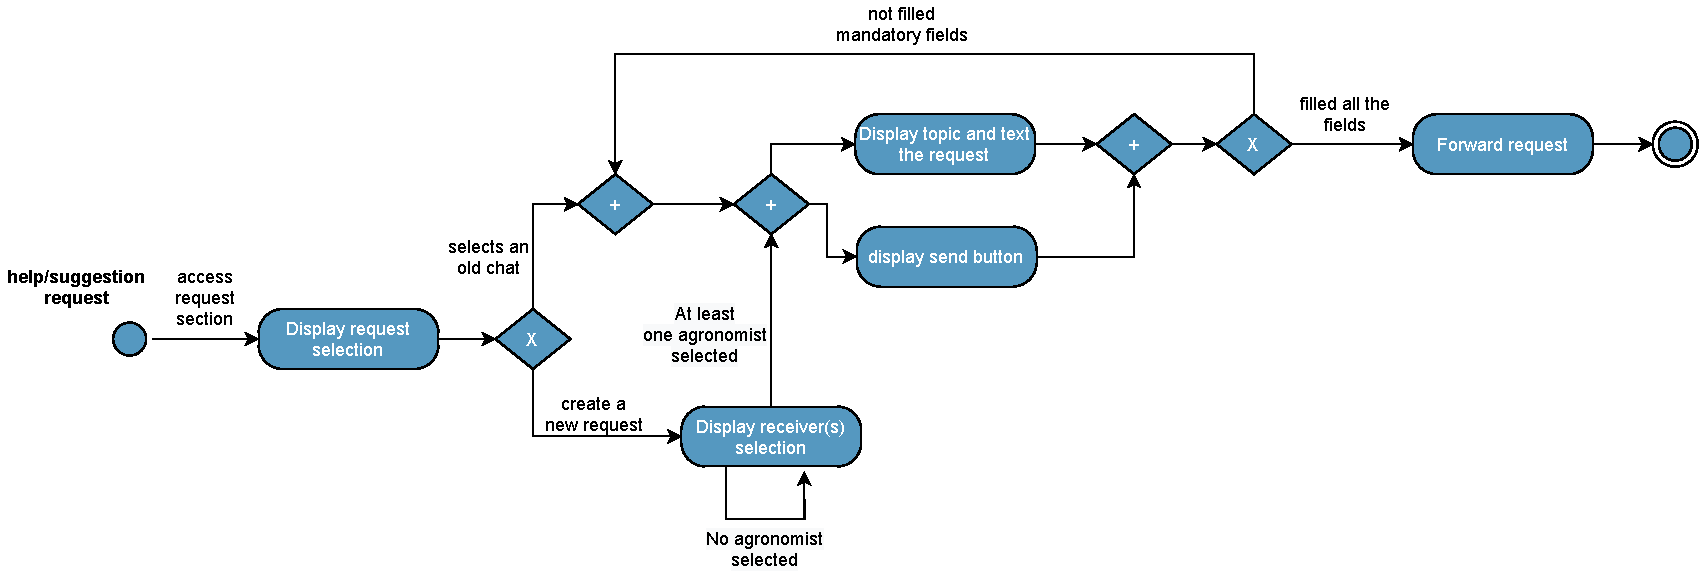
\includegraphics[width=\textwidth]{Images/BPMN/help-suggestion-request.pdf}
	\caption{\label{fig:bpmn_forum_generation}BPMN diagram of forum generation}
\end{figure}


\subsubsection{Visits to low performing farmers}
This functionality is necessary to organize the visits in order to make the schedule well-shared between an agronomist and a farmer. The agronomist goes to the daily plan section and the application displays a visualize or update button. If it is clicked, the system extracts their schedule data which is shortly expressed by a form with day-month-year and the farmers to visit.
If there is a wish to modify the plan, it is possible to modify it in a form guided by selecting the update button.

\begin{figure}[H]
	\centering
    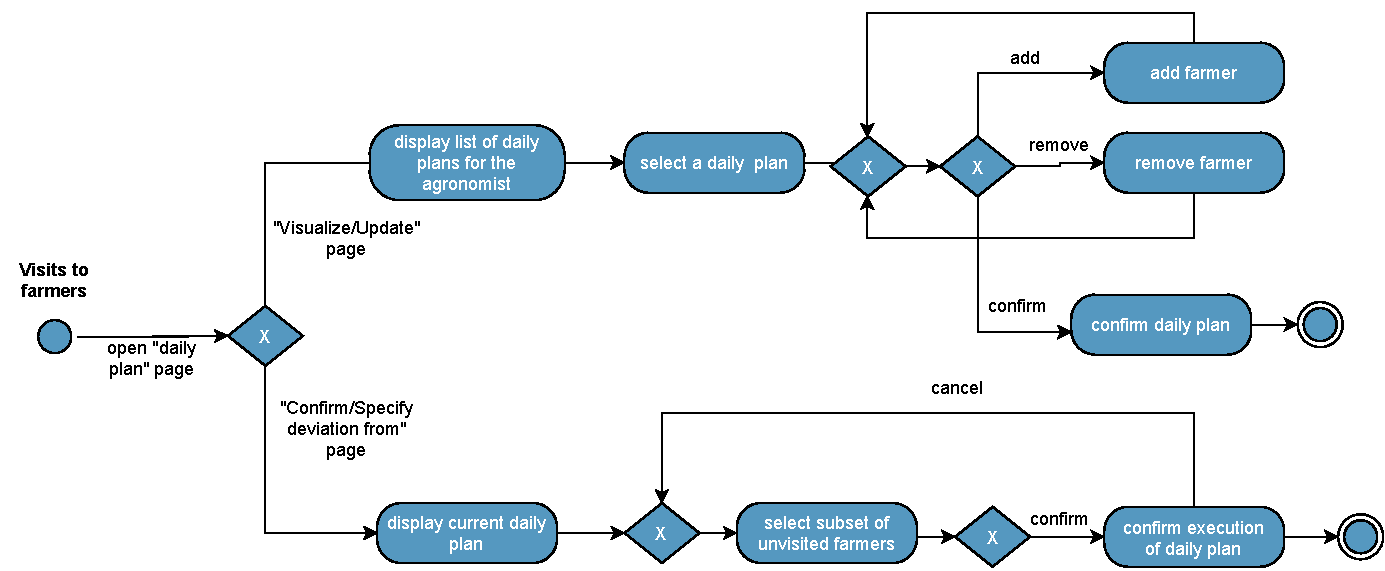
\includegraphics[width=\textwidth]{Images/BPMN/visit.pdf}
	\caption{\label{fig:bpmn_visit}BPMN diagram of visit farmers}
\end{figure}


\subsubsection{Visualize data about performance}
This functionality is used by policy makers. The policy maker clicks the farmer's performance button and the system visualize the list of farmers grouped by their production performance. If there is any interesting farmer, by selecting his/her name, the application shows the information of his/her production history.

\begin{figure}[H]
	\centering
    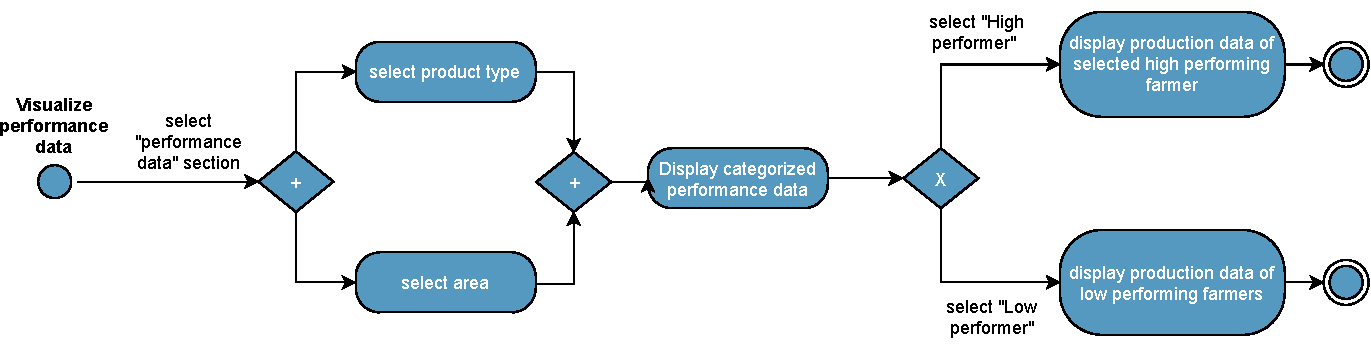
\includegraphics[width=\textwidth]{Images/BPMN/Performance.pdf}
	\caption{\label{fig:bpmn_performance}BPMN diagram of farmer performance}
\end{figure}

\subsection{Actors}
\label{sec:actors}
In this section are defined the professional figures which, according to the assignment, the system will interact with: \textbf{policy makers}, \textbf{farmers} and \textbf{agronomists}. In order to avoid redundancy, we also introduce the concept of \textbf{user} as an abstract entity that collects their common properties. As shown in figure \ref{fig:uml_class_diagram}, they inherit user's properties.
\subsubsection{User}
It is a person who wants to use the service. In order to access the system, it has to register to the platform (the first time) and be logged in (the following times). It also requires an Internet connection to properly use the system.
\subsubsection{Policy maker}
It is someone interested in the overall performing situation of Telangana’s farmers (e.g., Telangana’s government). It is able to surf on \hyperref[tab:acronymsTable]{DREAM}’s website. It uses the service to visualise information about well and under-performing farmers and to understand if the steering initiatives are producing significant results.
\subsubsection{Farmer}
It is a farmer of Telangana. It is able to surf on \hyperref[tab:acronymsTable]{DREAM}’s website (or to use the smartphone application). It uses the service in order to discuss with other farmers, to send requests for help to an agronomist, to insert product information, to know when it will receive a visit from an agronomist. It takes advantage in using the system because it can receive incentives if it is well-performing or can receive help if it is under-performing.
\subsubsection{Agronomist}
It is an agronomist of Telangana. It is able to surf on \hyperref[tab:acronymsTable]{DREAM}’s website (or to use the smartphone application). It uses the service to answer farmers' requests for help, to visualise data concerning their areas (weather forecasts, well and under-performing farmers, problems encountered by farmers), to visualise and update a daily plan to visit farms in the area, to confirm the execution or specify deviation from the daily plan.

\newpage

\subsection{Assumptions, dependencies and constraints}
\label{sec:domain_assumptions}
In this section we present the assumptions that are expected to hold in the world, the part of the environment that the machine cannot perceive nor control. The satisfaction of these so called \textbf{domain assumptions} are deeply related to the reliability of the system to behave in the expected way. If at least one of these assumptions is discovered not to be guaranteed, then the expected behaviour of the machine would allow the occurrence of an unstable state of the machine with unpredictable results.
\newline

\begin{table}[H]
    \setlength\arrayrulewidth{1pt}
    \centering
    \rowcolors{2}{white}{myblue!25}
    \begin{tabular}{|l|m{0.85\textwidth}|}
        \rowcolor{myblue}
        \hline
        \color{white}DX & \color{white}Definition \\
        \hline
        \textsc{D1}  &    Data concerning meteorologial short-term and long-term forecasts is exact and reliable \\
        \hline
        \textsc{D2}     &   Information obtained by the water irrigation system is reliable \\
        \hline
        \textsc{D3}  &    Information on the humidity of soil obtained by sensors deployed on the territory is reliable\\
        \hline
        \textsc{D4}  &    Each user who wants to use the online service (web page, app) must have a device connected to Internet\\
        \hline
        \textsc{D5}  &    Information inserted in the system by agronomists is reliable\\
        \hline
        \textsc{D6}  &    Information stored in the systems by farmers is reliable (e.g. farmers do not insert false data about their production or their problems to look better/worse performing)\\
        \hline
        \textsc{D7}  &    The analysis about how good a farmer is doing is reliable\\
        \hline
        \textsc{D8}  &    The user is supposed to be at least 18 years old\\
        \hline
        \textsc{D9}  &    The analysis on good farmers will be used by the Government to calculate the special incentives \\
        \hline
        \textsc{D10}     &   The special incentives given by the Government are well-proportioned and reliable \\
        \hline
        \textsc{D11}  &    The comparison of the current performance with past history is reliable\\
        \hline
        \textsc{D12}  &    Each user who wants to use the online service (web page, app) must have a device connected to Internet\\
        \hline
        \textsc{D13}  &    When a problem occurs, farmers insert that information in the system\\
        \hline
        \textsc{D14}  &    When an agronomist plans the visits of a daily plan, most farmers will be present\\
        \hline
        \textsc{D15}  &    Agronomists will always confirm the execution (specifying deviations, if needed) of the daily plan at the end of the same day\\
        \hline
        \textsc{D16}  &    An agronomist is responsible for just one area\\
        \hline
        \textsc{D17}  &    Farmers usually interact with the system (periodic product information upload, checking for agronomist visits) \\
        \hline
        \textsc{D18}     &   When a farmer starts a forum thread, a reply will be given as soon as possible \\
        \hline
        \textsc{D19}  &    The categorized weather types provided by a third party analysis are reliable\\
        \hline
        \textsc{D20}  &    Observation of  farmers' performance is done frequently by policy makers\\
        \hline
        \textsc{D21}  &    Policy maker has enough information and knowledge to understand the proper moment to ask for good practices\\
        \hline
        \textsc{D22}  &    Outstanding high performing farmers are asked by policy makers to write their good practices periodically\\
        \hline
        \textsc{D24}  &    Farmer agrees on allowing the system to store information about them (location of the activity, information on production, ...)\\
        \hline
        
    \end{tabular}
    
    \caption{\label{tab:domainAssumptions}Table of domain assumptions}
    
\end{table}

\tmref{link to traceability matrix}